\section{Prototype}
% TODO: How does the prototype handle sample quality?
%           - Length of clips?
%           - Performed in quiet environment?
Due to the findings in the analysis section, the prototypes scope has been
limited to feature extraction from the different sensors in the watch. This means
that no feature comparison will be performed. This was found to be a necessary
compromise, as all the proposed systems requires advanced machine learning to
function optimally. An implementation of the \textit{Dynamic Time Warp}
algorithm has also been included, to test if any comparison algorithm is
possible on a smart watch \cite{berndt1994using}.
Much of the code has been inspired by open source examples 
\cite{watchosheartratesamplerepo} \cite{healthkitheartrateexporter} 
\cite{watchossampler}, found on the popular code repository site \textit{GitHub}.
The main purpose of the prototype is therefore to sample the sensors, allowing
for further analysis of the output.

The prototype includes feature extraction from the three possible sensors,
    i.e.\ the microphone, accelerometer and heart rate sensor. These should be
easily sampled, and extracted from the device, this process will also be
covered. 

\subsection{User Interface}
The developed user interface found in figure~\ref{fig:ui}, allows the wearer
to perform measurements with the watch. This includes samples of
heart rate, voice and movement. Testing of the \textit{Dynamic Time Warping} has
also been included, which involves running \textit{DTW} on a two arrays of
length 1000.
The different samplings can be configured upon spawning of their views, this is
done from the main views controller, \texttt{MainInterfaceController}, see
listing~\ref{lst:ui}.

\begin{lstlisting}[label={lst:ui}, caption={Spawning of ViewControllers from the
main interface, passing contexts setting up the sampling.},basicstyle=\small]
@IBAction func movementButtonTapped() {
    let context = MovementInterfaceContext()
    context.instruction = "Sampling Movement"
    context.dataStorePath = "Movement_sample_\(NSTimeIntervalSince1970).data"
    context.sampleDuration = 10.0
    context.completionClosure = {() -> Void in print("Done")}
    self.pushControllerWithName("movementScene", context: context)
}

@IBAction func voiceButtonTapped() {
    let context = VoiceInterfaceContext()
    context.instruction = "Sampling Voice"
    context.dataStorePath = "Voice_sample_\(NSTimeIntervalSince1970).mp4"
    context.sampleDuration = 10.0
    context.completionClosure = {() -> Void in print("Done")}
    self.pushControllerWithName("voiceScene", context: context)
}

@IBAction func heartRateButtonTapped() {
    let context = HeartRateInterfaceContext()
    context.instruction = "Sampling Heart"
    context.dataStorePath = "HeartRate_sample_\(NSTimeIntervalSince1970).data"
    context.sampleDuration = 100.0
    context.completionClosure = {() -> Void in print("Done")}
    self.pushControllerWithName("heartRateScene", context: context)
 }

@IBAction func dtwTestButtonTapped() {
    let context = DynamicTimeWarpInterfaceContext()
    context.instruction = "Testing DTW"
    context.testSampleSize = 1000
    self.pushControllerWithName("dtwScene", context: context)
}
\end{lstlisting}


\begin{figure}[!h]
\centering
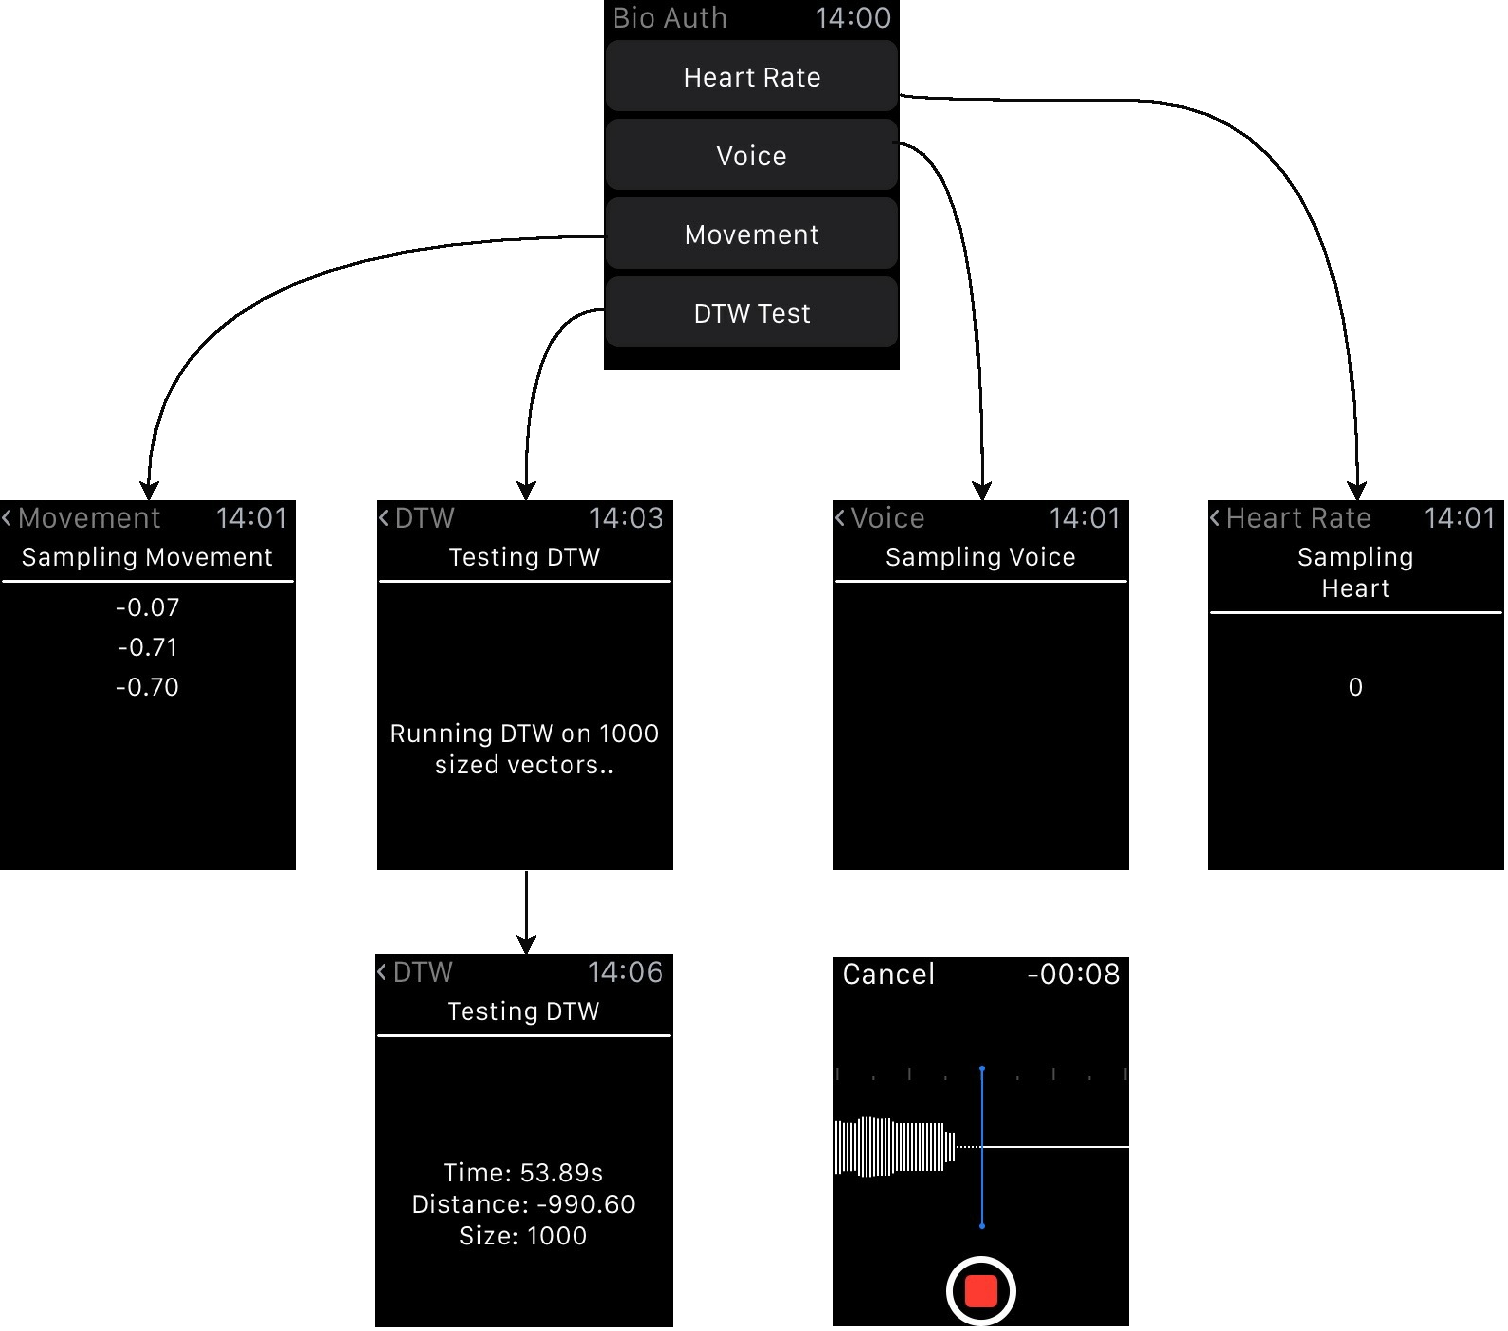
\includegraphics[width=1.0\textwidth]{../media/bioswp_ui.pdf}
\caption{Flow of the developed prototypes user interface. Start menu allows for
data extraction from the three sensors and to run DTW on arrays with 1000
    entries.}
\label{fig:ui}
\end{figure}

\subsection{Microphone}
All functionality related to the microphone is handled by the microphone view,
which is controlled by the \texttt{VoiceInterfaceController}.
Here the recording interface is spawned to record the specified time. The
recording can be performed in a variety of qualities and formats, and is spawned
with the \texttt{WKInterfaceController} function
\texttt{presentAudioControllerWithOutputURL}, see listing~\ref{lst:rec}. The format is
controlled by the file extension on the \texttt{NSURL} which the function saves
the recording to, and the quality is defined in the \texttt{preset}. The
different presets can be found in table~\ref{tbl:rec}.

\begin{lstlisting}[label={lst:rec}, caption={Spawning of the audio recording
    controller.},basicstyle=\small]
self.presentAudioRecorderControllerWithOutputURL(
    recFileUrl,
    preset: WKAudioRecorderPreset.WideBandSpeech,
    options: [
        WKAudioRecorderControllerOptionsMaximumDurationKey: 
            NSTimeInterval(duration)
    ],
    completion: { (didSave, error) -> Void in
        print("error: \(error)\n")
        if didSave {
            self.storeVoiceData(toFile, dataUrl: recFileUrl)
            self.popController()
        } else { self.popController() }
})
\end{lstlisting}

\begin{table}[!h]
\caption{Available audio recording presets, their sampling rate and bit rate.}
\label{tbl:rec}
\centering
\begin{tabular}{ |l|l|l|  }
\hline
\multicolumn{3}{|c|}{Audio Recorder Presets} \\
\hline
Preset             & Sample Rate & Format / Bit Rate\\
\hline
HighQualityAudio   & 44.1 kHz    & LPCM 705.6 kbps or AAC 96 kbps \\
WideBandSpeach     & 16 kHz      & LPCM 256 kbps or AAC 32 kbps \\
NarrowBandSpeach   & 8 kHz       & LPCM 128 kbps or AAC 24 kbps \\
\hline
\end{tabular}
\end{table}

\subsection{Accelerometer}


\subsection{Heart Rate Sensor}

\subsection{Dynamic Time Warp}
The implementation of DTW is only included to showcase the computation power of
the \textit{Apple Watch}, and to evaluate if it is viable to run such a rather
heavy algorithm on the watch.
The DTW algorithm has beenMotion Sensors implemented in the class
\texttt{DynamicTimeWarper}. The class only has a single function,
    \texttt{distance}, which takes to arrays of doubles, and returns the
    calculated distance between the two. The algorithm is run by the
    \texttt{DynamicTimeWarpInterfaceController}, which tracks how long time the
    algorithm takes to execute the algorithm, on arrays filled with random data. 
As seen in table~\ref{tbl:dtw} the complexity is as expected $O(n^2)$.
This makes it viable to run smaller sets with this algorithm, and other distance
measuring algorithms could probably also run on the device.
Another approach could be to execute the algorithm on the connected iPhone,
which would result in a significant performance boost, due to the more powerful
hardware. This would allow for more complex algorithms on largers sets of data.


\begin{lstlisting}[label={lst:dtw},caption={Testing of the implemented DTW
    algorithm, within the DynamicTimeWarpInterfaceController}]
dispatch_async(queue) {
    let dtw = DynamicTimeWarper()
    let testArr1 = (0...localContext.testSampleSize!).map {_ in drand48()}
    let testArr2 = (0...localContext.testSampleSize!).map {_ in drand48()}
    let distance = String(format: "%.2f", dtw.distance(testArr1, target: testArr2))
    let deltaTime = String(format: "%.2f", abs(self.dtwStart!.timeIntervalSinceNow))
    self.resultLabel.setText("Time: \(deltaTime)s\n
                              Distance: \(distance)\n
                              Size: \(localContext.testSampleSize!)")
}
\end{lstlisting}

\begin{table}[!h]
\caption{Measure time it takes to run DTW on different sized arrays.}
\label{tbl:rec}
\centering
\begin{tabular}{ |c|c|  }
\hline
Array Size  & Time in seconds\\
\hline
100    &        \\
250    &        \\
500    &        \\
1000   & 53.89  \\
\hline
\end{tabular}
\end{table}

\subsection{Data transfer and storage}

